\documentclass[]{article}
\usepackage{lmodern}
\usepackage{amssymb,amsmath}
\usepackage{ifxetex,ifluatex}
\usepackage{fixltx2e} % provides \textsubscript
\ifnum 0\ifxetex 1\fi\ifluatex 1\fi=0 % if pdftex
  \usepackage[T1]{fontenc}
  \usepackage[utf8]{inputenc}
\else % if luatex or xelatex
  \ifxetex
    \usepackage{mathspec}
  \else
    \usepackage{fontspec}
  \fi
  \defaultfontfeatures{Ligatures=TeX,Scale=MatchLowercase}
\fi
% use upquote if available, for straight quotes in verbatim environments
\IfFileExists{upquote.sty}{\usepackage{upquote}}{}
% use microtype if available
\IfFileExists{microtype.sty}{%
\usepackage{microtype}
\UseMicrotypeSet[protrusion]{basicmath} % disable protrusion for tt fonts
}{}
\usepackage[unicode=true]{hyperref}
\hypersetup{
            pdfborder={0 0 0},
            breaklinks=true}
\urlstyle{same}  % don't use monospace font for urls
\usepackage{graphicx,grffile}
\makeatletter
\def\maxwidth{\ifdim\Gin@nat@width>\linewidth\linewidth\else\Gin@nat@width\fi}
\def\maxheight{\ifdim\Gin@nat@height>\textheight\textheight\else\Gin@nat@height\fi}
\makeatother
% Scale images if necessary, so that they will not overflow the page
% margins by default, and it is still possible to overwrite the defaults
% using explicit options in \includegraphics[width, height, ...]{}
\setkeys{Gin}{width=\maxwidth,height=\maxheight,keepaspectratio}
\IfFileExists{parskip.sty}{%
\usepackage{parskip}
}{% else
\setlength{\parindent}{0pt}
\setlength{\parskip}{6pt plus 2pt minus 1pt}
}
\setlength{\emergencystretch}{3em}  % prevent overfull lines
\providecommand{\tightlist}{%
  \setlength{\itemsep}{0pt}\setlength{\parskip}{0pt}}
\setcounter{secnumdepth}{0}
% Redefines (sub)paragraphs to behave more like sections
\ifx\paragraph\undefined\else
\let\oldparagraph\paragraph
\renewcommand{\paragraph}[1]{\oldparagraph{#1}\mbox{}}
\fi
\ifx\subparagraph\undefined\else
\let\oldsubparagraph\subparagraph
\renewcommand{\subparagraph}[1]{\oldsubparagraph{#1}\mbox{}}
\fi

% set default figure placement to htbp
\makeatletter
\def\fps@figure{htbp}
\makeatother


\date{}

\begin{document}

\section{(sezione) Esempi di quesiti a scelta multipla
(QSM)}\label{sezione-esempi-di-quesiti-a-scelta-multipla-qsm}

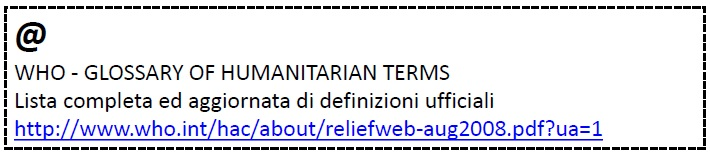
\includegraphics[width=3.45278in,height=2.58333in]{media/image1.jpeg}

La Sindrome NIMBY si riferisce a delle opere ritenute utili ma, con un
approccio egoistico, non volute nelle vicinanze di residenza delle
persone interessate. (Risposta corretta: D)

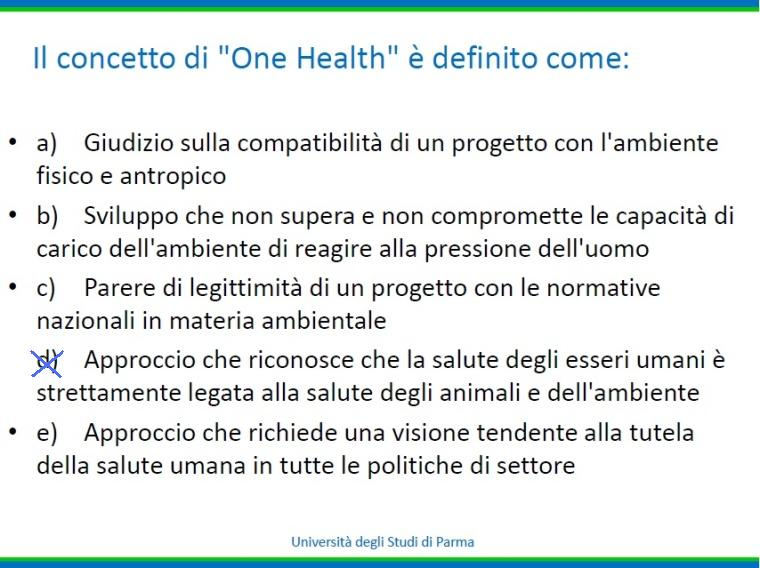
\includegraphics[width=3.45278in,height=2.58333in]{media/image2.jpeg}

(Risposta corretta: D)

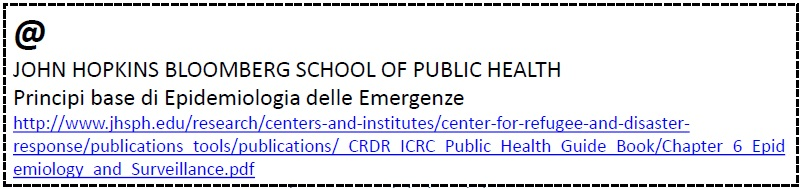
\includegraphics[width=3.52083in,height=2.63425in]{media/image3.jpeg}

Per quanto quello di \textless{}\textless{}Health in all
polices\textgreater{}\textgreater{} sia un concetto assolutamente logico
e che risuona nella teoria, nella pratica delle politiche non sanitarie
(ambientali, sociali, economiche) è in realtà di difficile applicazione,
in quanto entrano in gioco altri interessi che sono in conflitto con
l'interesse della tutela della salute. (Risposta corretta: E)

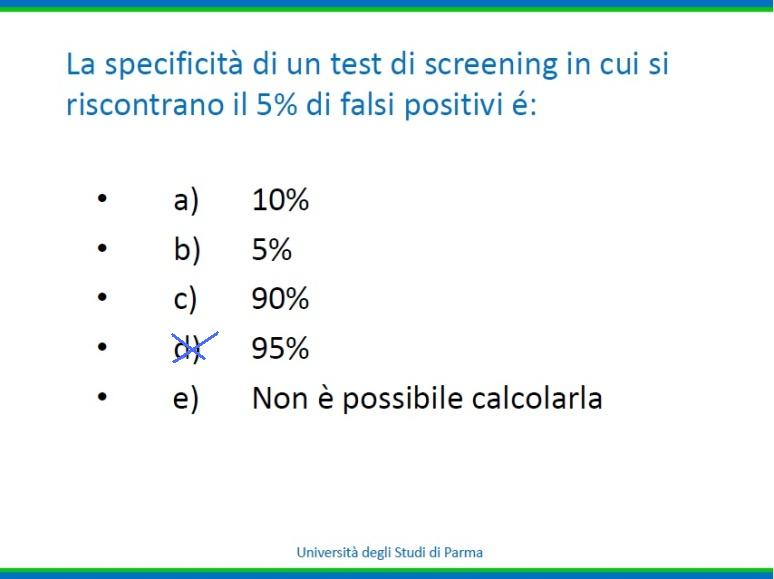
\includegraphics[width=3.52083in,height=2.63460in]{media/image4.jpeg}

La sezione dedicata allo screening è un argomento d'esame ricorrente sia
nei quiz che nell'esame orale, in quanto argomento cardine della sanità
pubblica, della prevenzione e dell'epidemiologia. è importante conoscere
le definizioni e saper calcolare specificità, sensibilità, valore
predittivo positivo e valore predittivo negativo. (Risposta corretta: D)

Un'altra domanda ricorrente riguarda quale dei due gruppi (sensibilità e
specificità o valori predittivi positivo e negativo) è influenzato dalla
prevalenza di una malattia. Ad essere influenzati dalla prevalenza sono
i valori predittivi (che cambiano valore a seconda di quanto sia
prevalente la malattia) mentre specificità e sensibilità non lo sono.

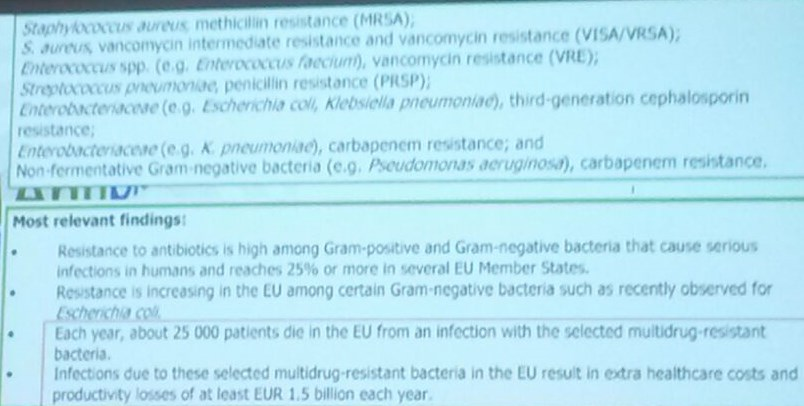
\includegraphics[width=3.52083in,height=2.63460in]{media/image5.jpeg}

(Risposta corretta: A)

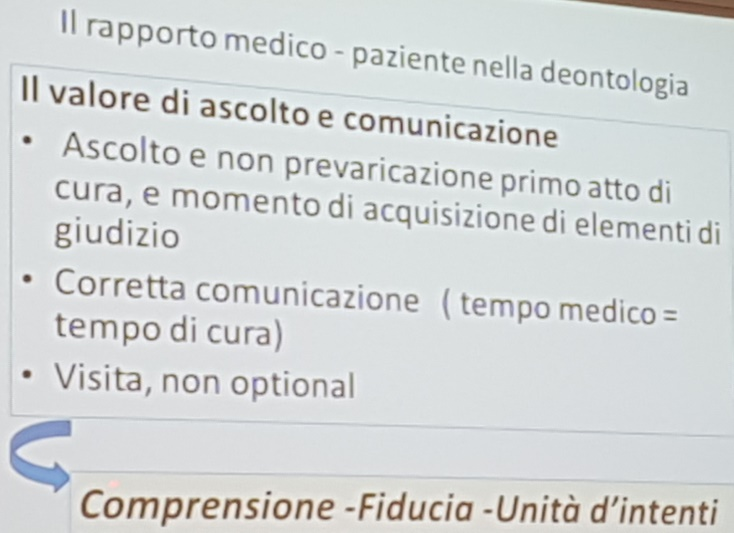
\includegraphics[width=3.52193in,height=2.63542in]{media/image6.jpeg}

(Risposta corretta: C)

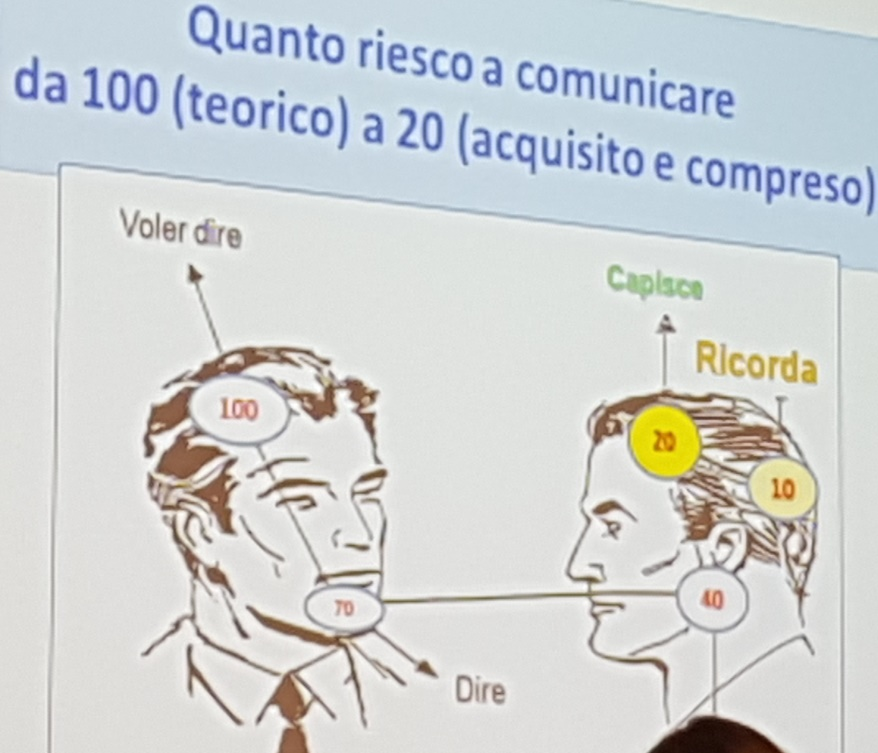
\includegraphics[width=3.52083in,height=2.63460in]{media/image7.jpeg}

(Risposta corretta: E) La risposta A è la definizione di Advocacy.

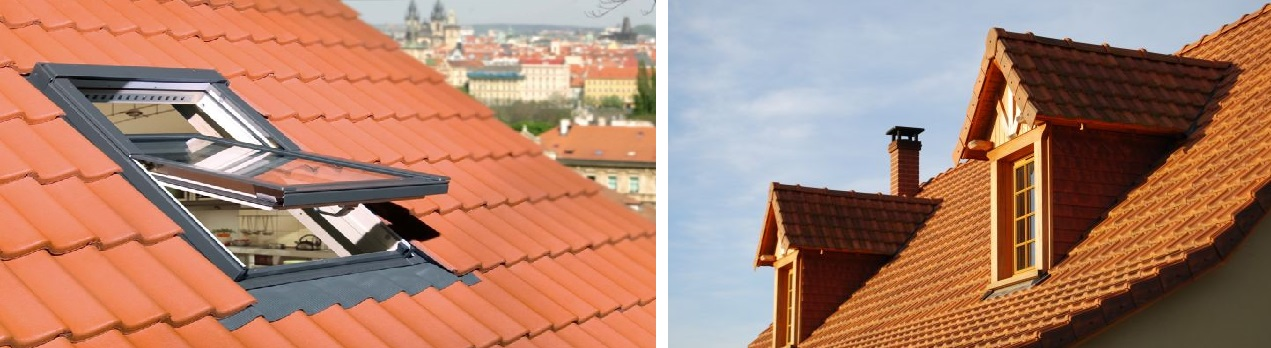
\includegraphics[width=3.52083in,height=2.63460in]{media/image8.jpeg}

(Risposta corretta: B)

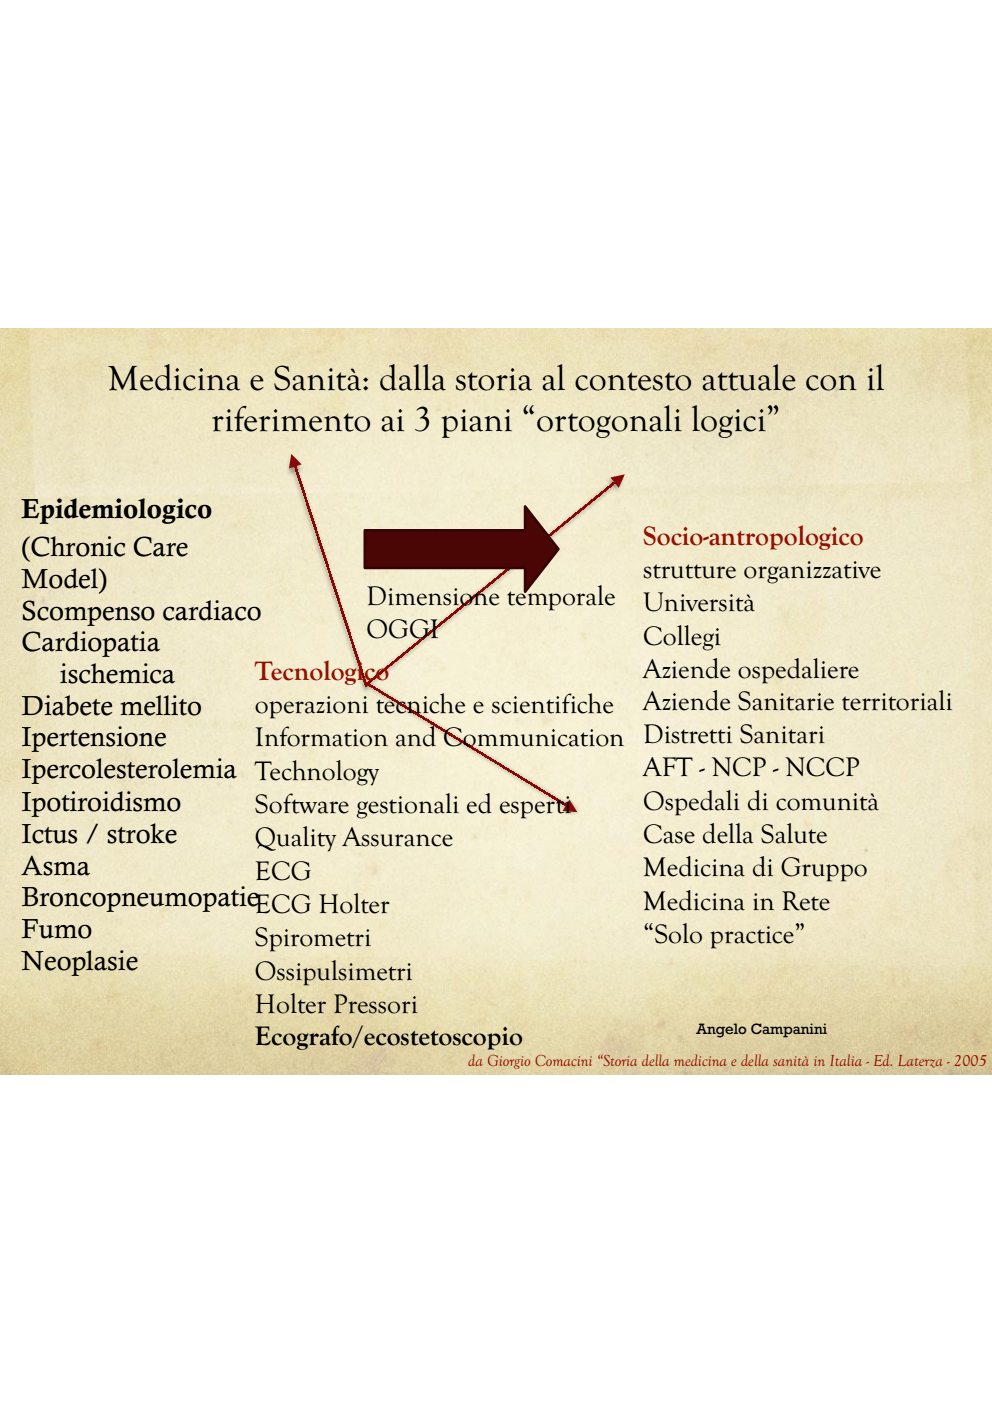
\includegraphics[width=3.53634in,height=2.64583in]{media/image9.png}

(Risposta corretta: A)

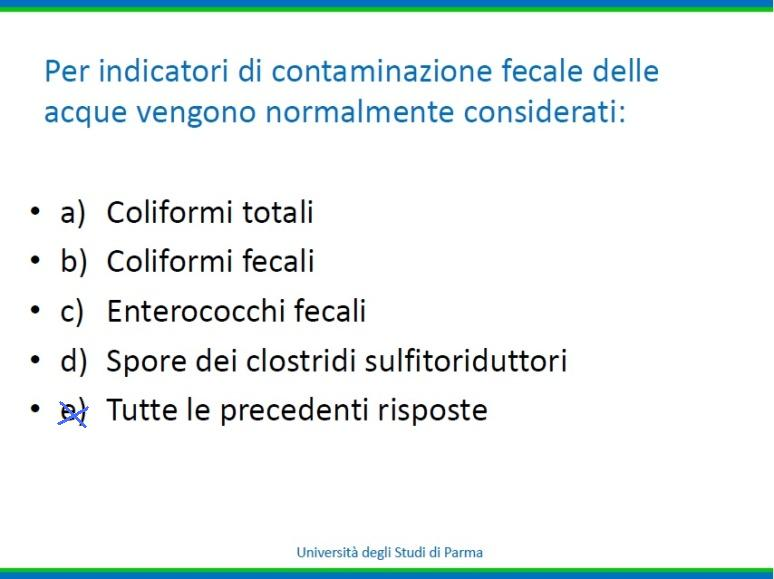
\includegraphics[width=3.52083in,height=2.63460in]{media/image10.jpeg}

(Risposta corretta: E)

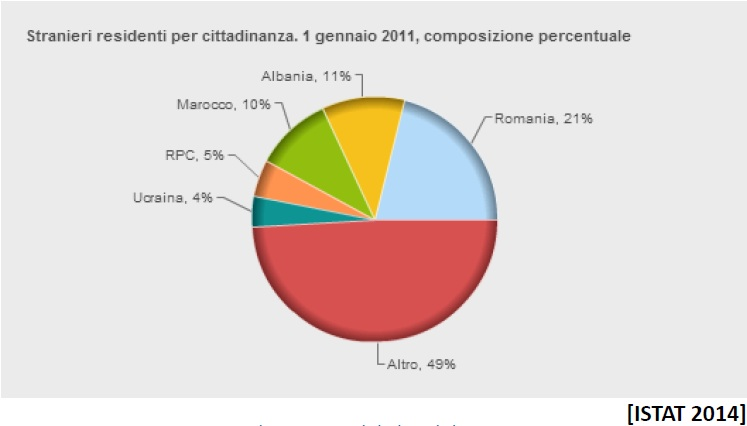
\includegraphics[width=3.60545in,height=2.69792in]{media/image11.jpeg}

Fare attenzione alla differenza tra infezione alimentare e tossinfezione
alimentare in quanto cambiano i microorganismi, i tempi di incubazione e
di conseguenza le misure di profilassi e di prevenzione. (Risposta
corretta: A)

\end{document}
